% -*-latex-*-
% Document name: /Users/nbrouard/Documents/COURS/iford/manuscrit-iford/corrigé-TD2-fev-1984.tex
% Creator: Nicolas J Brouard  [nbrouard@tugault.ined.fr]
% Creation Date: Sun Jan  7 16:17:26 2018


% These lines tell TeXworks to typeset with xelatex, and to open and
% save the source with Unicode encoding.
% !TEX program = xelatex
% !TEX encoding = UTF-8 Unicode
%\documentclass{memoir}
%\documentclass[11pt,a4paper]{amsart}
\documentclass[11pt,letterpaper]{article}
\scrollmode
%\usepackage{mathptmx} % This if you want Times Roman fonts.
%\usepackage{fontspec} % for xetex and luatex engines
%\usepackage[utf8x]{inputenc} %for pdftex engine and unicode characters
%\usepackage[latin1]{inputenc} % for pdftex engine and iso-8859-1 characters
%\usepackage[T1]{fontenc} % for pdftex and Cork fonts (extended CMR fonts)
\usepackage{hyperref} %\href{url}{label} or \url{url}
\usepackage{amsmath,xcolor}
%\usepackage{amsmath,amsthm,txfonts,color}
%\usepackage{mathmacr}
%\usepackage{anysize}\marginsize{0.2cm}{0.2cm}{0.2cm}{0.2cm}
%\usepackage[landscape,twocolumn, top=3cm, bottom=5cm, left=1cm, right=1cm]{geometry}
%\usepackage[landscape,twocolumn]{geometry}
%\usepackage{fullpage}
%\usepackage[2cm]{fullpage}
%\usepackage[french,english]{babel}
\usepackage{polyglossia}
%\setdefaultlanguage{french}
\setmainlanguage{english}
\setotherlanguage{french}
\usepackage{graphicx}
%\usepackage{doublespace,endfloat} % Put figure and table at the end
%\usepackage{fapalike} % Put the bibliography as apa
%\usepackage{natbib} % Put the bibliography as apa
%\makeatletter \renewcommand{@biblabel}[1]{} makeatother
\newcommand*{\doi}[1]{\href{http://dx.doi.org/\detokenize{#1}}{doi:
    \detokenize{#1}}}
\def\D{{\,\mathrm d}}
%\DeclareMathOperator{\D}{d}
\usepackage{geometry}
\geometry{top=2cm, bottom=5cm, left=2cm , right=2cm}
%\tolerance 200  % Standard TeX tolerance; could be set to 1000
\tolerance 1000  % Standard TeX tolerance; could be set to 1000
%\hyphenpenalty=100000
\hyphenpenalty=10
\emergencystretch=10pt
% %\usepackage{paracol} 
%\floatpagefraction .5
%\renewcommand{\floatpagefraction}{.9}
% \renewcommand{\topfraction}{0.9}	% max fraction of floats at top
% \renewcommand{\bottomfraction}{0.8}	% max fraction of floats at bottom
% \renewcommand{\dbltopfraction}{0.9}	% fit big float above 2-col. text
% \renewcommand{\textfraction}{0.07}	% allow minimal text w. figs
%  % Parameters for FLOAT pages (not text pages):
% \renewcommand{\floatpagefraction}{0.7}	% require fuller float pages
%      % N.B.: floatpagefraction MUST be less than topfraction !!
%\showthe\dblfloatpagefraction
\renewcommand{\dblfloatpagefraction}{0.7}	% require fuller float pages default 0.5
% % \newif\ifparacol
% % \paracoltrue
% % \columnratio{0.52}
\usepackage[yyyymmdd,hhmmss]{datetime}
%\ifparacol\showthe\hyphenpenalty\else\showthe\tolerance\fi
\bibliographystyle{natbib}
%\tolerance 200  % Standard TeX tolerance; could be set to 1000
%\floatpagefraction .5
%\enlargethispage{-\baselineskip} % squeeze one line
%\enlargethispage*{\baselineskip} % squeeze as much as possible
%\author{? \and ?}
%\usepackage[yyyymmdd,hhmmss]{datetime}
%\date{\today \,at \currenttime}
%\date{}
% mathmacr.sty  N. Brouard 4/02/88
\def\relstack#1#2{\mathrel{\mathop{#1}\limits_{#2}}}
\def\D{{\,\mathrm d}}
%\def\e{{\,\mathrm e}}
%\def\E{{\,\mathrm E}}
\DeclareMathOperator{\e}{e}
\DeclareMathOperator{\E}{E}
\DeclareMathOperator{\Res}{Res}
%\newcommand{\E}{\DeclareMathOperator{\E}{E}}
\DeclareMathOperator{\Log}{Log}
\def\Pr{{\,\mathrm Pr}}
%\def\Log{{\,\mathrm Log\,}}
\def\Ln{{\,\mathrm Ln\,}}
%\def\ln{{\,{\mathrm ln}\,}}
\def\logit{{\,\mathrm logit\,}}
\DeclareMathOperator{\Var}{Var}
\DeclareMathOperator{\Ei}{Ei}
\DeclareMathOperator{\Eis}{Eis}
\DeclareMathOperator{\expint}{expint}
\DeclareMathOperator{\En}{En}
\DeclareMathOperator{\Eone}{E1}
%\def\Var{{\,{\mathrm Var}\,}}
%\def\Ei{{\,\mathrm Ei\,}}
%\def\Eone{{\,\mathrm E1\,}} % be careful with numbers!
%\def\En{{\,\mathrm En\,}}

  \begin{document}
% \bibliographystyle{fplain}
% \bibliographystyle{fapalike}
% \bibliographystyle{apalike}
% \bibliographystyle{apa}
% \bibliographystyle{plainnat}
% \makeatletter \renewcommand{\@biblabel}[1]{} \makeatother
% % \begin{paracol}{2}
% %     \selectlanguage{french}
% % \switchcolumn
% %     \selectlanguage{english}
\section*{Exercise }
Let us consider a population of women aged 50+ from the Health and
Retirement Study from 2009 to 2012 (Dudel C, Myrskyl ̈a M (2017)
Working life expectancy at age 50 in the united states and the impact
of the great recession. Demography 10.1007/s13524-017-0619-6, URL
https://doi.org/10.1007/s13524-017-0619-6). According to this
cross-longitudinal survey the authors estimated the age-specific forces of
transition between four states, employed, unemployed, inactive,
retired and death.

We are assuming that these 10 forces are varying by age but are constant
over time~\ref{f:forces-employment}.
 \begin{figure}[htbp]\centering
   %\vspace{4cm}
   %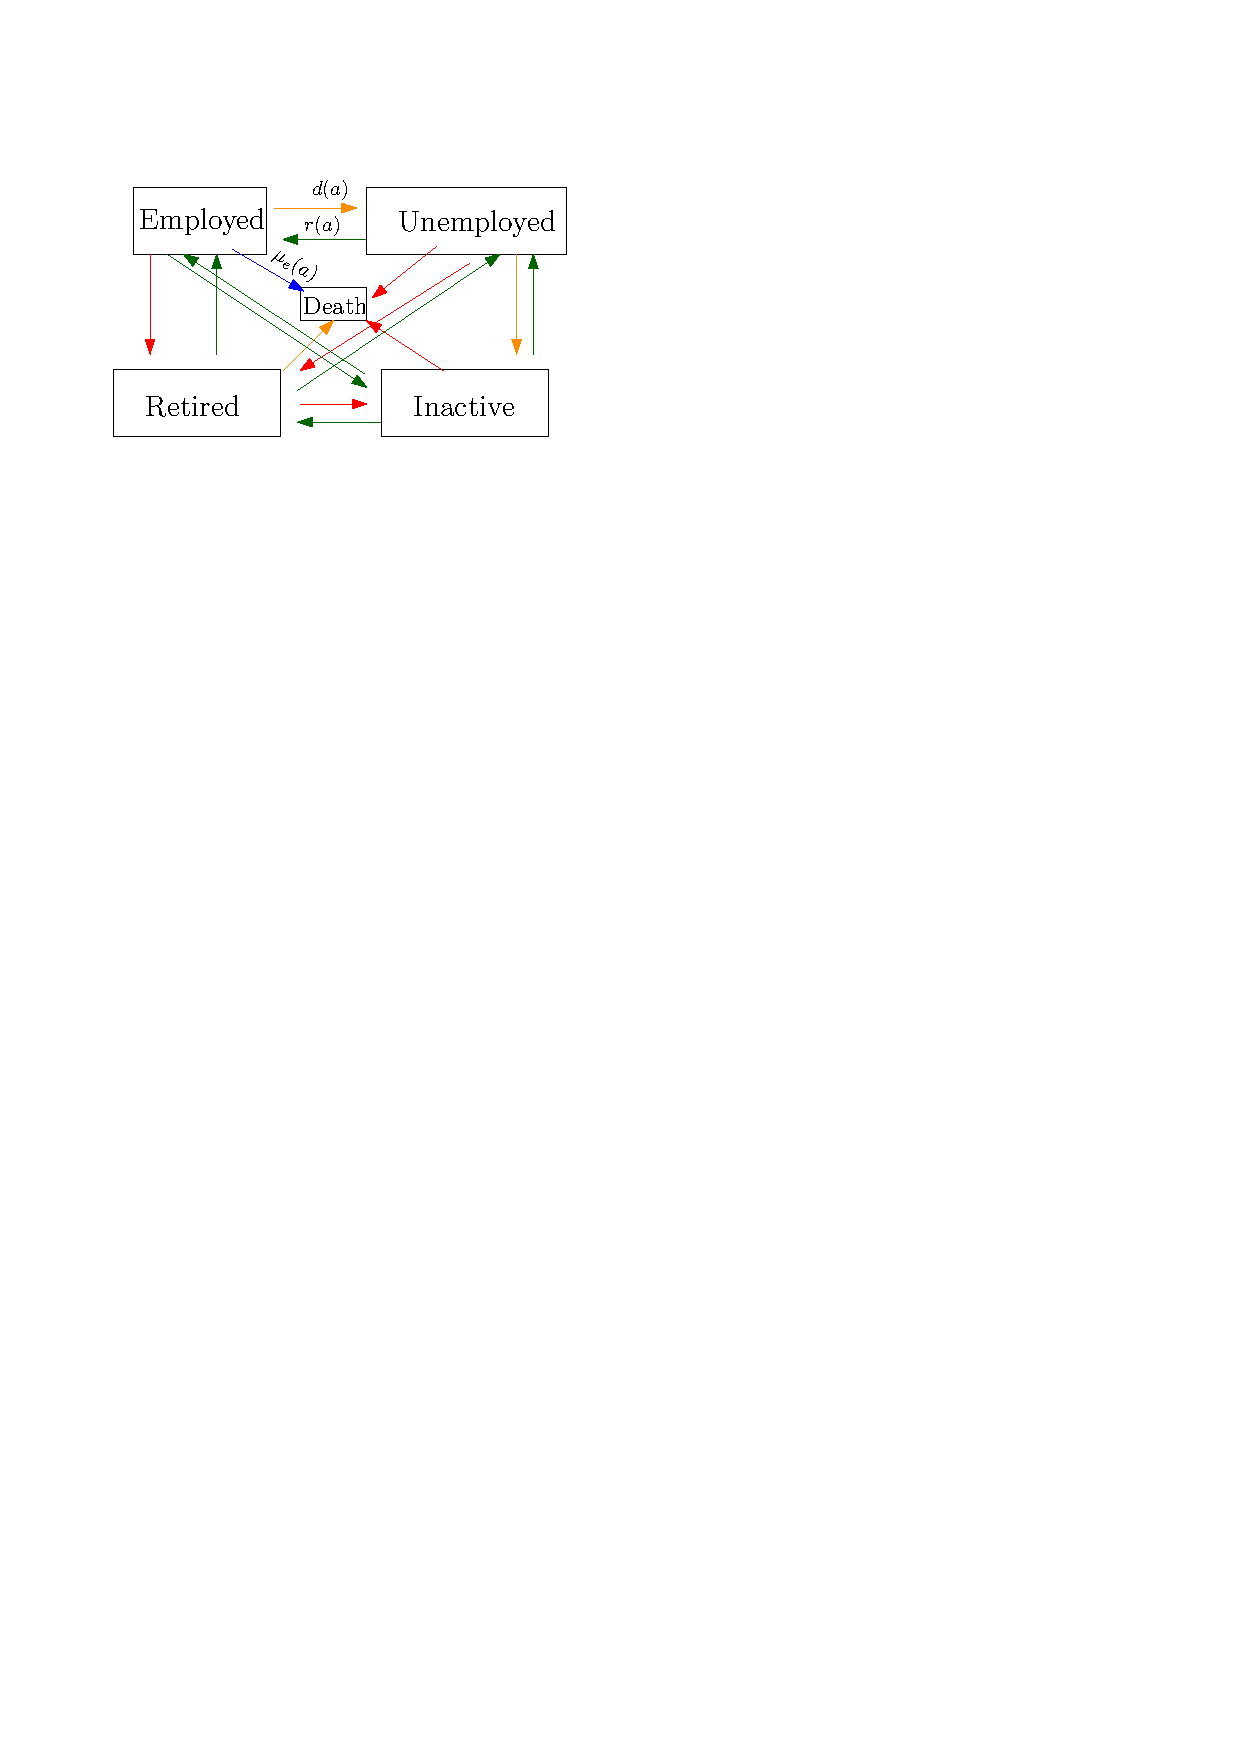
\includegraphics[width=.8\textwidth,height=.4\textheight]{forces-employment}
   %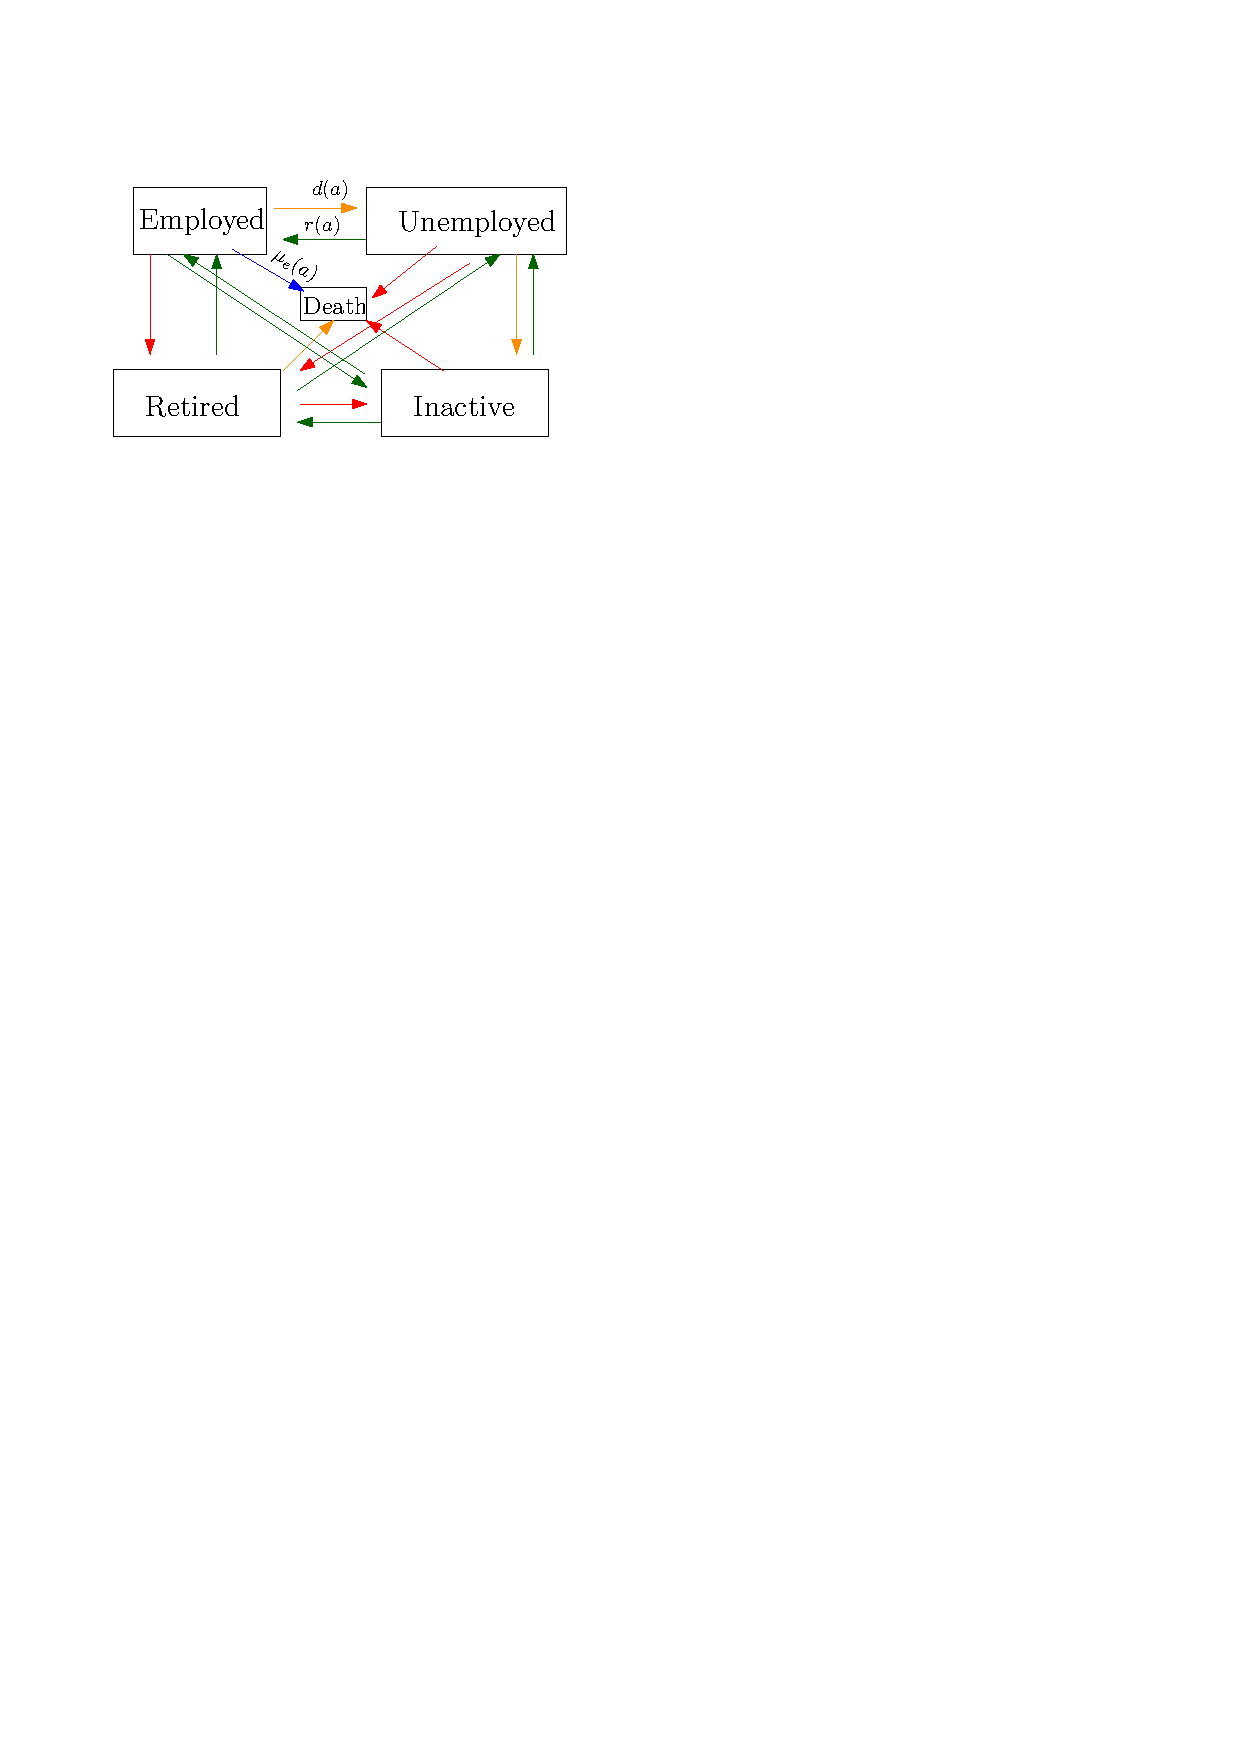
\includegraphics{forces-employment}
   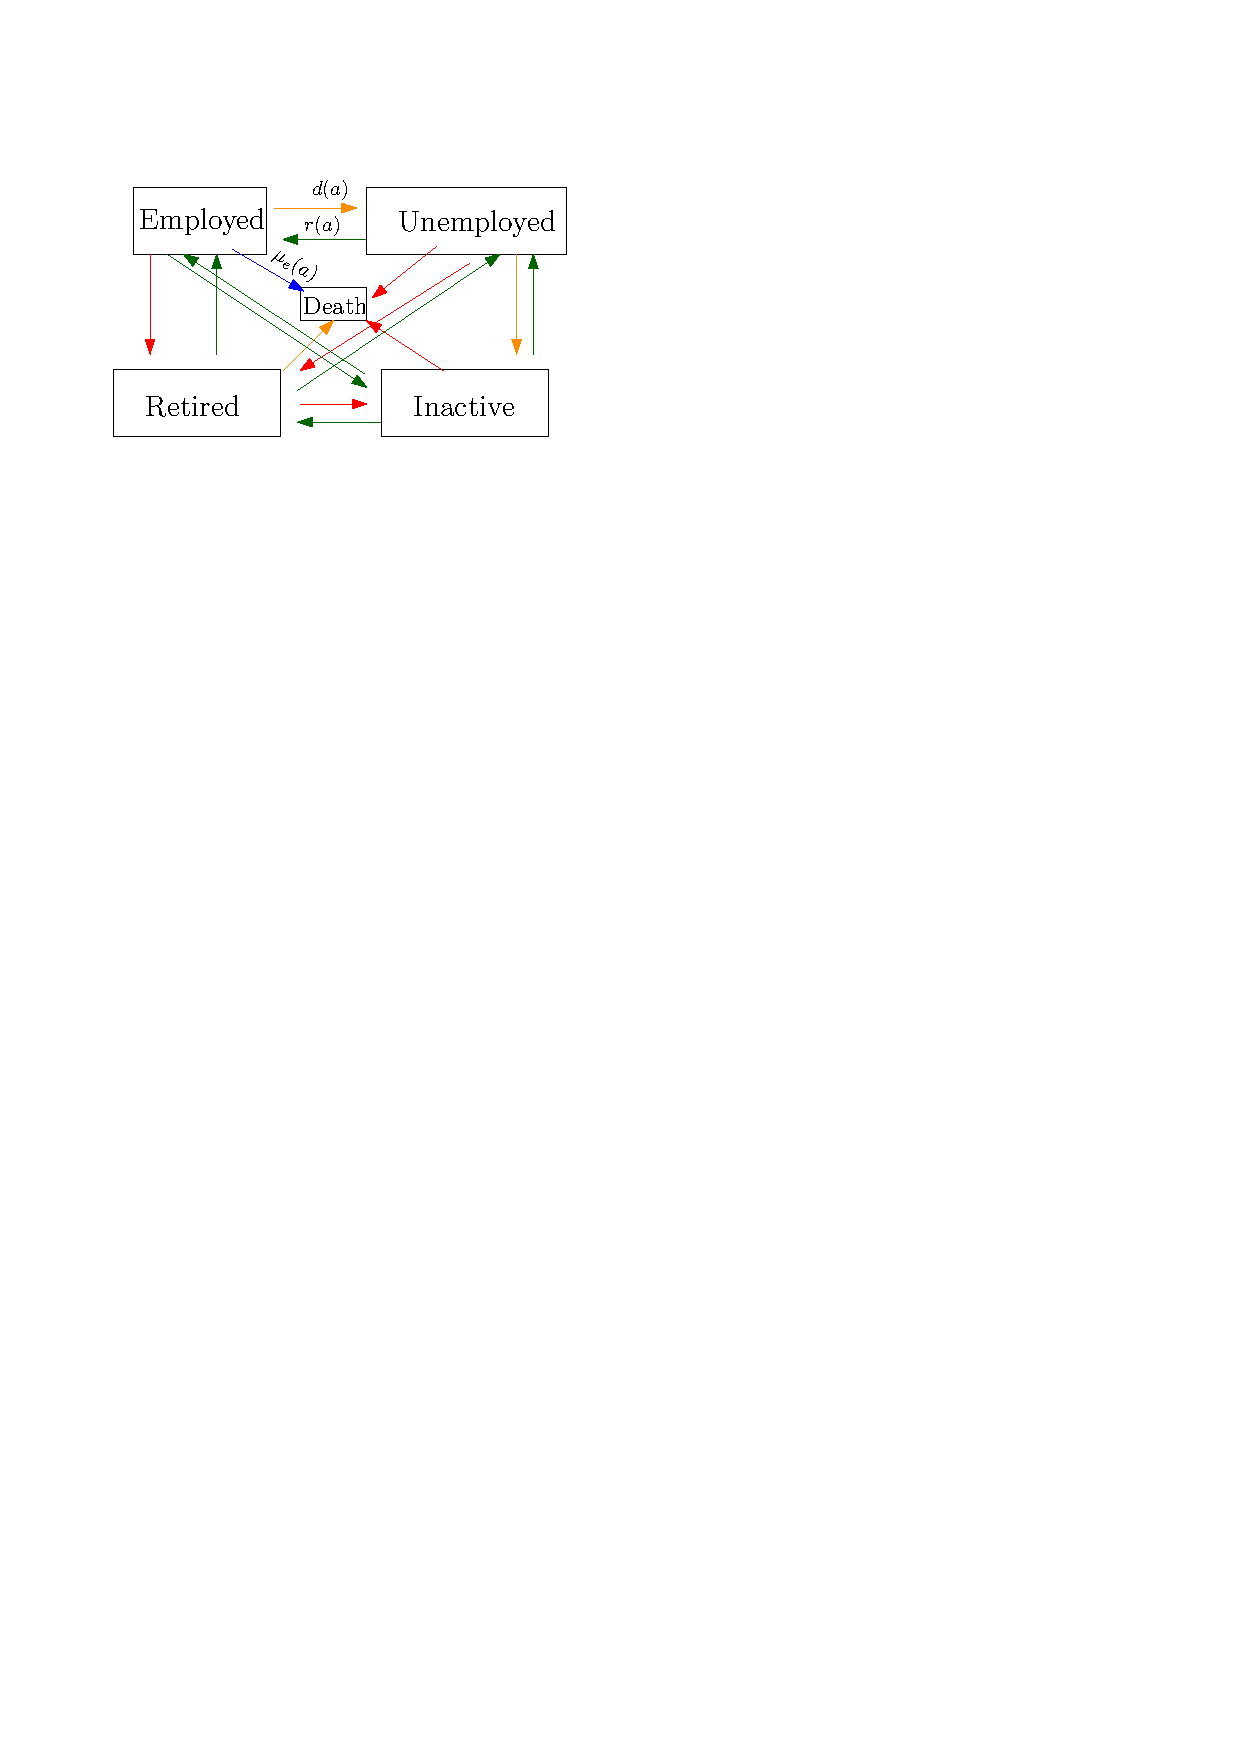
\includegraphics[width=.5\textwidth]{forces-employment}
   %\resizebox{.4\textwidth}{!}{\input{forces-employment}}   
   \caption{\sf States and age-specific forces. }\label{f:forces-employment}
 \end{figure}
The stationary multistate model is defined here by
supposing a constant flow of new women, just turning age 50, with a
fixed proportion in each of the 4 alive states.


\begin{enumerate}
\item \emph{Prove that the age specific prevalence in each state at
    time $t$ is constant over time.}  According to the property of
  continuous Markov processes, in each cohort, the proportion of women
  reaching any age is deterministic. And thus, cross-sectionally, at
  any time the proportion of women at any age is equal to the
  proportion in a single cohort.

  Let us detail the proof starting from the theory of Markov chain. We are assuming that
  an individual is jumping from state $i$ to $j$ each year. If we
  start from a cohort aged 50, by multiplying age specific matrices $P_x$, we
  get the proportion of women at each age until extinction by death.

  It is easy to generalize the definition, by permitting any transition
  within a year and thus, $P_x$ is now defined as the matrix of probabilities $_{1}P^{ij}_x$
  \emph{to be observed} in state $j$ at age $x+1$ being in state $i$
  at age $x$.
  \begin{align*}
    _{h}P_x &= \prod_{x=50}^{x+h} P_x
  \end{align*}

  Let us now consider a Lexis diagram and let $p(t,x)\D t$ be the population of women entering
  exact age $x$ between time $t$ and time $t+ \D t$.
  More precisely, let $p_s(t,x)\D t$ be the part of this population
  being in state $s$
  \begin{align*}
    p(t,x)\D t &= \sum_{s=1}^{4} p_s(t,x) \D t
  \end{align*}

  If the process starts at age 50 with $ p_s(t,50) \D t$ women in each
  state $s$, the multiplication of Markov matrices gives the
  corresponding probability to reach any age $x$ or, equivalently, the number of
  women to be expected in each state $s$ at age $x$ after $x-50$ steps.

  A simple generalization is to suppose that the Markov model is no
  more defined by year but by a smaller time, like a semester, trimester,
  month, wek, day or even a second. At the limit, it is called a Markov process.

  The age at start can also be continuous and thus the matrix $_hP_x$
  is the matrix of probabilities for a woman in state $i$ at age $x$ to be in
  state $j$ at age $x+h$.

 
  Thus from a cohort of women aged $x$ between time $t$ and $t+\D t$,
  the expected number reaching age $x+h$ between instants $t+h$ and
  $t+h+\D t$
  \begin{align*}
       p(t+h,50+h)\D t &= \prod_{x=50}^{x+h} P_x p(t,x) \D t
  \end{align*}
  
  Let us now consider a stationary process defined by a constant flow
  $p_s(t,x) \D t$ of women in state $s$ reaching age $50$ between any
  elapsed time $\D t$.  This flow is also equal to the number of women
  observed at exact time $t$ and aged between $50$ and $50+\D t$ (see
  Brouard 1989). This might be defined as the population density of a
  multistate stationary population in state $s$, at time $t$ and age
  $x$.


  
  
\item \emph{At time $t$, let us now classify the population in state $s$ according to the
     last period spent in that state. Let $Z_s(t,d)$ be the pyramid
    by duration $d$ (number of women having been continously in state
    $s$ since less than $d$ time) at time $t$. Prove that the function
    $Z_s(t,d)$ is independent of time $t$,is a decreasing function
    and that the total population $Z(t,d)=Z(d)=\sum_{d=1}^4 Z_s(d)$.}


  Let $Z_s(t,d)$ be, at time $t$ (see Fig:~\ref{f:exercise-multistate-lexis-ipe}),
 \begin{figure}[htbp]\centering
   %\vspace{4cm}
   %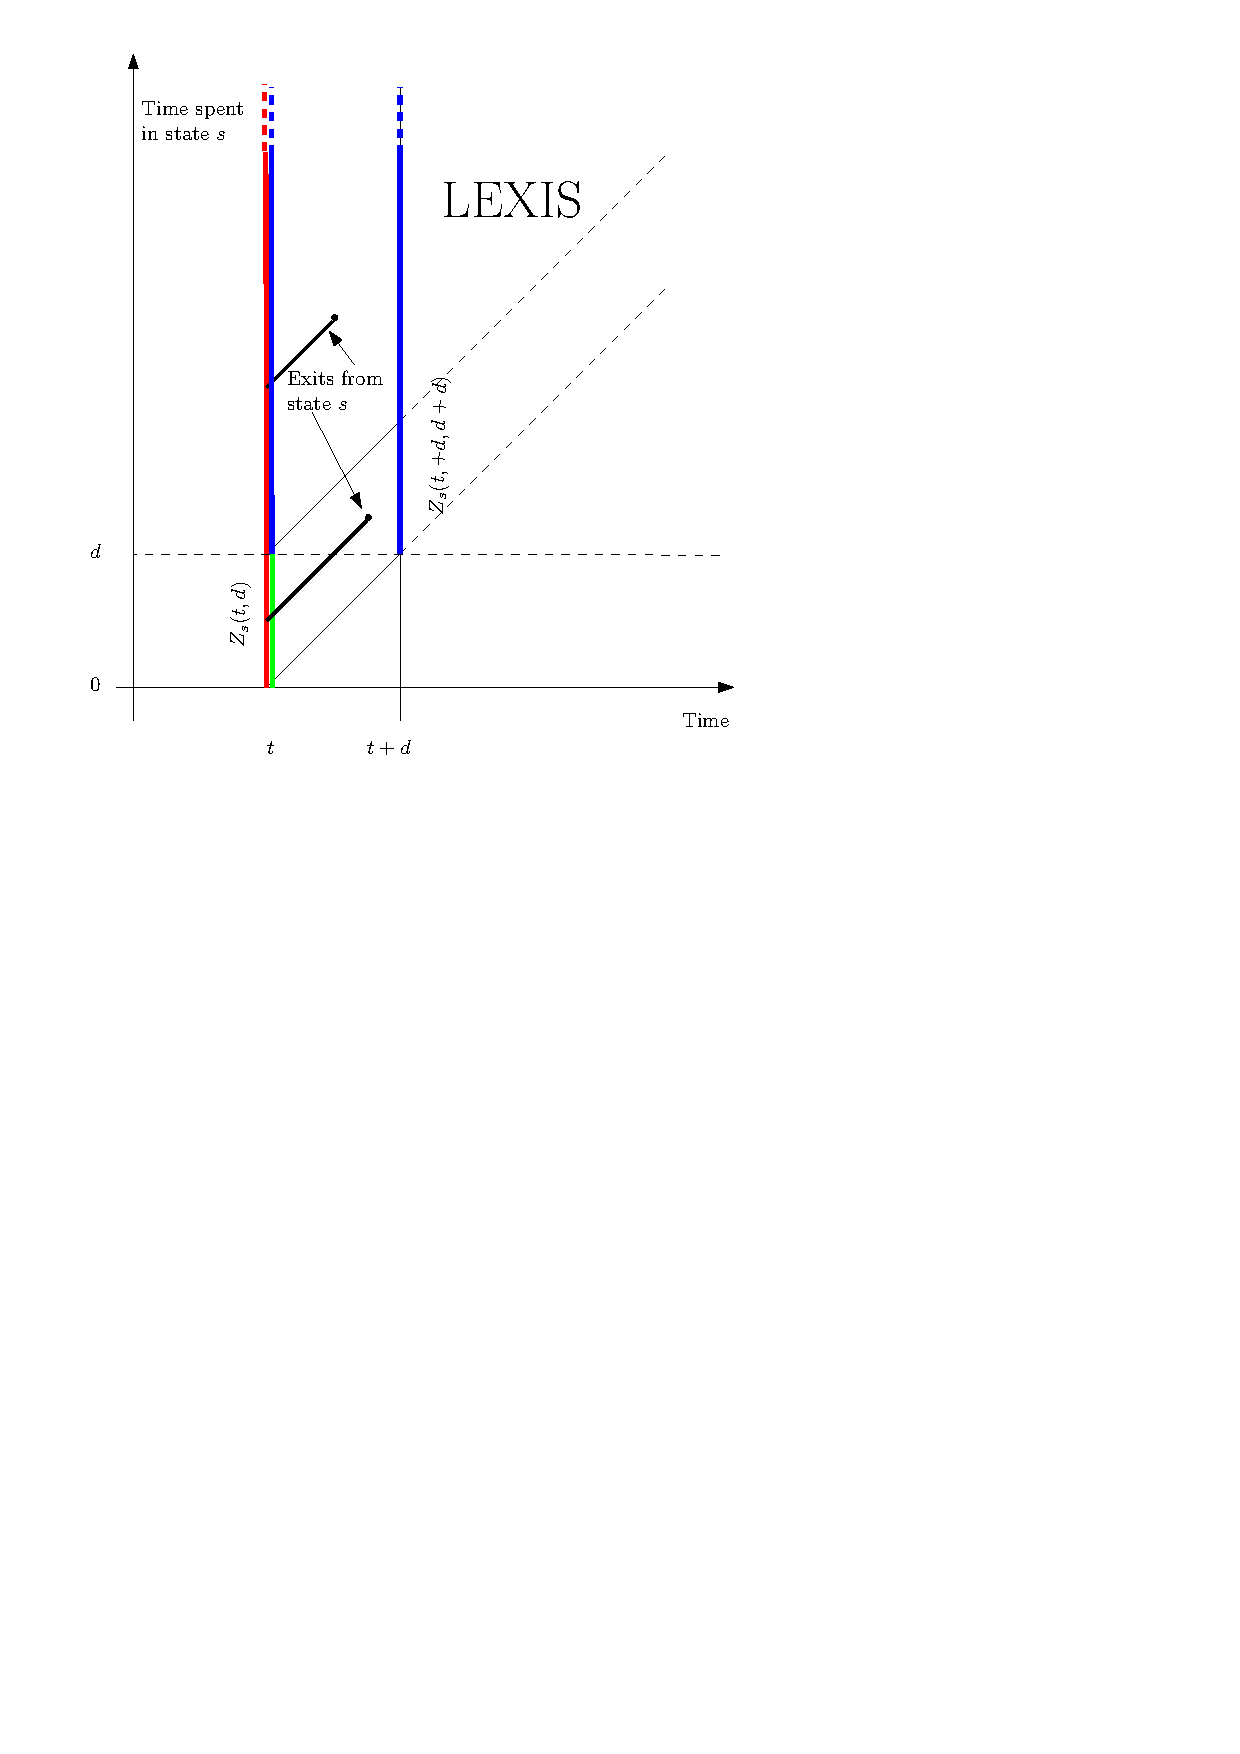
\includegraphics[width=.8\textwidth,height=.4\textheight]{exercise-multistate-lexis-ipe}
   %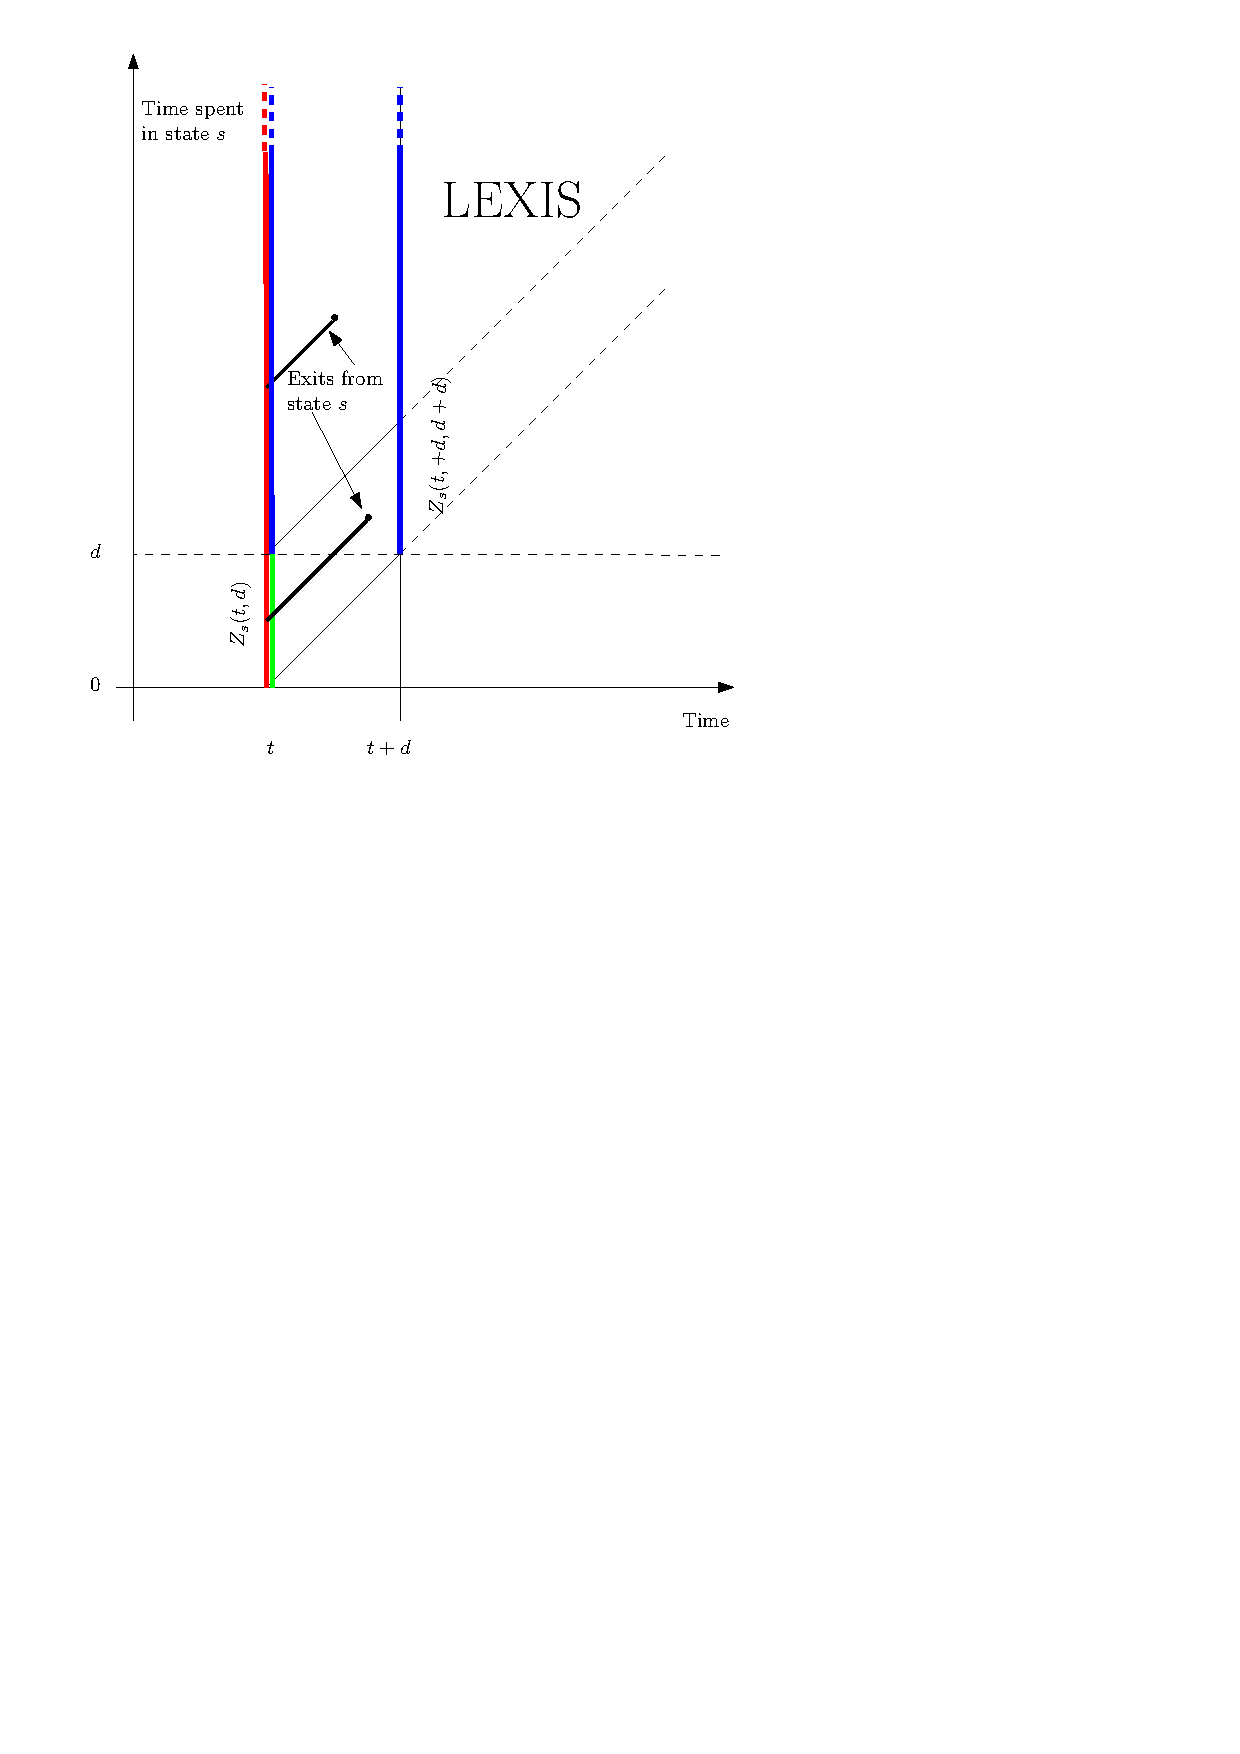
\includegraphics{exercise-multistate-lexis-ipe}
   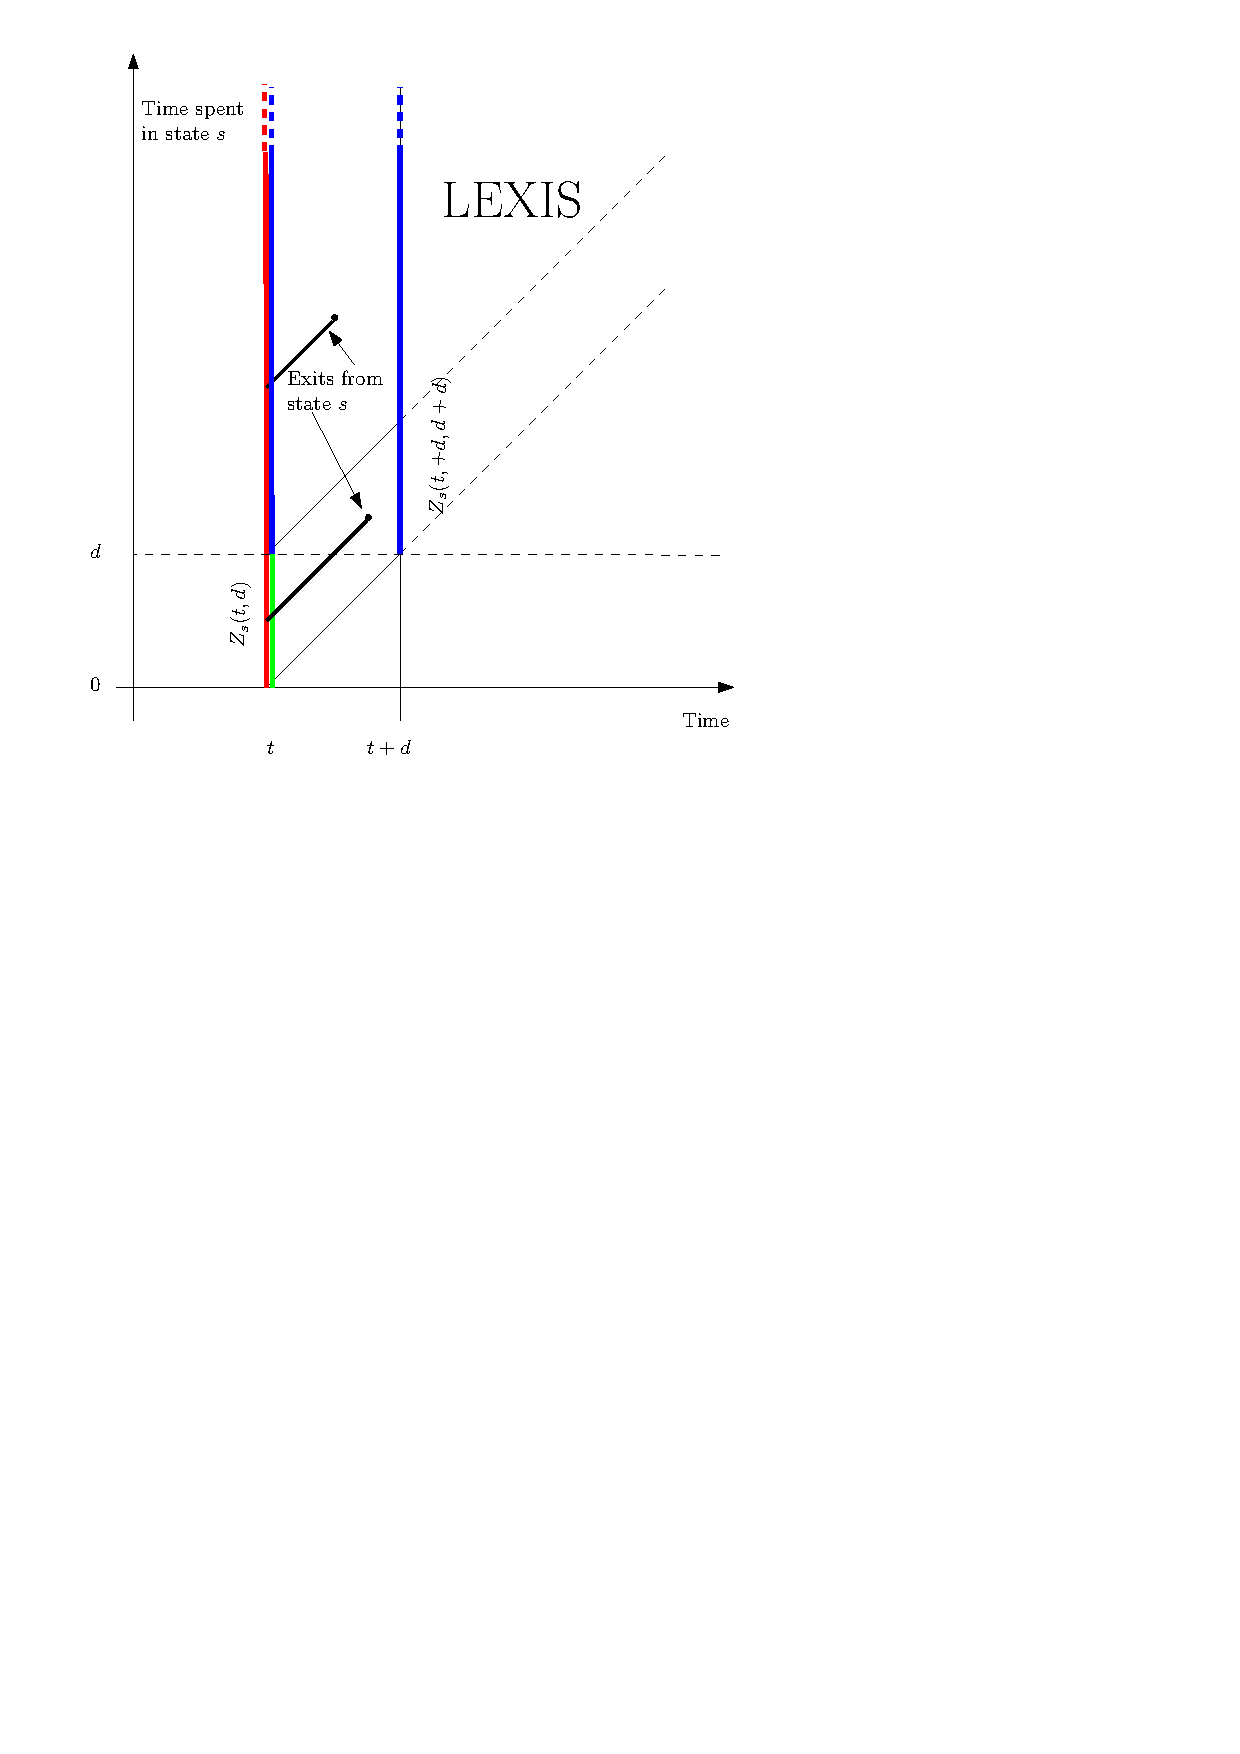
\includegraphics[width=.5\textwidth]{exercise-multistate-lexis-ipe}
   %\resizebox{.4\textwidth}{!}{\input{exercise-multistate-lexis-ipe}}   
   \caption{\sf Lexis diagram where age is replaced by the duration of
     the last period in state
     $s$. }\label{f:exercise-multistate-lexis-ipe}
 \end{figure}
 the total number of women having
  been continously in state $s$ since less than $d$ time (green segment). At time
  $t+d$, some women have left state $s$ and some remained in
  state $s$. Some leaved state $s$ to another state and returned to
  state $s$ but they do no more belong to the population having been
  continuously in state $s$. Thus,
  $Z_s(t,d) <= Z_s(t+d,d+d)$ which proves that the population
  is decreasing with time/duration.

\item \emph{ Among the $Z_s(t,d)$ women present at time $t$, how many of them
  will leave the state $s$ within the $d$ next years? Hint: Draw a
  Lexis diagram (time $t$ and duration $d$) and forecast the
  stationary population at time $t+d$, what is the difference between
  $Z_s(t+d,2d)-Z_s(t,d)$?}

If $Z_s(t,d)$ is the number of women having been constantly in state
$s$ since less than time $d$, the number of women at time $t+d$ having
been in state $s$ constantly between time $d$ and time $2d$, is
because of the stationarity $Z_s(t+d,2d)$. And the difference
$Z_s(t+d,2d)-Z_s(t,d)$ is simply the women who left state $s$ during
the period $t$ and $t+d$.

From the total population (red vertical segment from 0 to $+\infty$),
$Z_s(t,d+)$ is the population at time $t$ being in state $s$ during
more tha $d$ time (blue segment). Therefore, we have
$Z_s(t)=Z_s(t,d)+Z_s(t,d+)$\,. Only $Z_s(t+d,d+)$ will remain in state
$s$ at time $t+d$. And, because of the stationarity,
$Z_s(t+d,d+)=Z_s(t,d+)$ (number of women crossing the blue segments
are equal).  Therefore the number of women who left state $s$ is the
difference between the red and blue segment which is the green segment
$Z_s(t) - Z_s(t+d,d+)= Z_s(t,d)$.

\item \emph{ From the total population $Z(t)$ at time $t$ how many of
    them will leave the state $s$ within time $t$ and time $t+d$?}
  The property is that in a multistate stationary population, the
  number of women continuously in state $s$ since $d$ time is equal to
  the number of women who will stay continuoulsly $d$ time in state
  $s$ whatever $d$ is.

  
\item \emph{ Propose a method to have a fully stationary population, that is:
  what should be the prevalence at initial age 50 among the 4 alive
  states?}

\end{enumerate}

%\newpage
% % % \begin{paracol}{2}
% % %     \selectlanguage{french}
% % \switchcolumn
% %     \selectlanguage{english}
% % \section*{Exercise (corrected)}
% % \begin{enumerate}
% % \end{enumerate}
% % \end{paracol}
\end{document}

%
% These lines tells gnu-emacs to typeset with the xetex engine
% which requires Unicode encoding only (utf-8)
% ^c^t^s for toggling synctex. 
% ^-Shift-Click to move from pdf to source, Command-Shift-Click on OSX
%%% Local Variables:
%%% TeX-engine: xetex
%%% TeX-source-correlate-method-active: synctex
%%% ispell-local-dictionary: "american"
%%% coding: utf-8
%%% End:
